% Prämabel
\documentclass[11pt,a4paper]{article}

% Codage
\usepackage[utf8]{inputenc}
\usepackage[T1]{fontenc}
\usepackage{siunitx}
\usepackage{indentfirst}

% Langue
\usepackage[english]{babel}

% Supplément
\usepackage{amsmath,amsfonts,amssymb}
\usepackage{verbatim} % pour faire des commentaires avec \begin{comment}...
\usepackage{float} % pour positioner un image exacetement où on veut
\usepackage
  [separate-uncertainty = true,
  multi-part-units = repeat]
  {siunitx} % Exemple \SI{0}{\kg \cdot \m^{-3}}

% Images
\usepackage[pdftex]{graphicx}
\usepackage{graphics}
\usepackage{subcaption} % pour positioner des figures côte à côte
\usepackage{wrapfig}

% pour l'inclusion de liens dans le document 
\usepackage[colorlinks,bookmarks=false,linkcolor=blue,urlcolor=blue]{hyperref}


% la mise en page
\usepackage{geometry}
\paperheight=297mm
\paperwidth=210mm

\pagestyle{plain}



% nouvelles commandes LaTeX, utilis\'ees comme abreviations utiles
\newcommand{\mail}[1]{{\href{mailto:#1}{#1}}}
\newcommand{\ftplink}[1]{{\href{ftp://#1}{#1}}}

%%%%%%%%%%%%%%%%%%%%%%%%%%%%%%%%%%%%%%%%%%%%%%%%%%%%%%%%
\begin{document}


% Le titre, l'auteur et la date
\title{Numerical Exercise \#1}
\author{Caspar Gutsche\\  % \\ pour fin de ligne
}
\date{\today}
\maketitle
%%%%%%%%%%%%%%%%%%%%%%%%%%%%%%%%%%%%%%%%%%%%%%%%%%%%%%%%



\newpage
\section{Question \#1}
\begin{figure}[h]
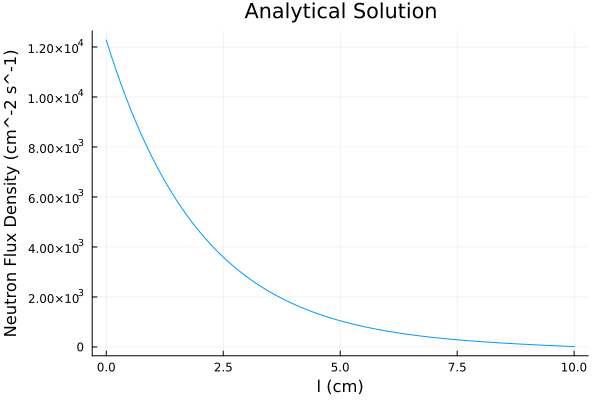
\includegraphics[width=7cm]{../figs/ex1_analytical.png}
\centering
\caption{Analytical Solution for the neutron flux as a function of depth.}
\end{figure}
Flux values at the following locations (4 significant digits):\\
Flux value at $x_0$: 13.589586060473522 $cm^-2 s^-1$\\
Flux value at $0^+$:12276.897875372839  $cm^-2 s^-1$ \\

% Φ(1.05 * u"cm") = 7329.878134314118 cm^-2 s^-1
% Φ(0 * u"cm") = 12276.897875372839 cm^-2 s^-1
% Φ(x0) = 13.589586060473522 cm^-2 s^-1

\section{Question \#2}

Relationship between $\mathrm{\Phi}_i,\ \mathrm{\Phi}_{i+1},\ \mathrm{\Phi}_{i-1}$ at any point within the material:
\begin{equation}
    \frac{1}{dx^2}(\Phi_{i-1} - 2 \Phi_{i} + \Phi_{i+1}) - \frac{1}{L} \Phi_{i} = 0
\end{equation}

Coefficients of the matrix A (4 significant digits), for a mesh size of 0.1cm:\\
Coef ${} A_{i,i} = -200.2411 cm^{-2}$: \\
Coef $A_{i-1,i} = 99.9999 cm^{-2}$: \\
Coef $A_{i+1,i} = 99.9999 cm^{-2}$: \\

Relationship between $\mathrm{\Phi}_i,\ \mathrm{\Phi}_{i-1/2},\ \mathrm{\Phi}_{i+1/2}$, \\
at the source:
\begin{align}
J_{x}^{+}\left( x_{n+\frac{1}{2}} \right) &= \frac{S}{2}  = \frac{1}{4}\Phi\left( x_{n+\frac{1}{2}} \right) - \frac{D}{2} \frac{d}{dx}\Phi  \\
        & = \frac{\Phi_{n+\frac{1}{2}}}{4}-\frac{D}{2} \frac{\Phi_{n+\frac{1}{2}}-\Phi_{n}}{\frac{dx}{2}} \\
\end{align}
at the RHS of the problem:
\begin{align}
    J_{x}^{-}\left( x_{n+\frac{1}{2}} \right) &= 0  = \frac{1}{4}\Phi\left( x_{n+\frac{1}{2}} \right) + \frac{D}{2} \frac{d}{dx}\Phi  \\
        & = \frac{\Phi_{n+\frac{1}{2}}}{4}+\frac{D}{2} \frac{\Phi_{n+\frac{1}{2}}-\Phi_{n}}{\frac{dx}{2}} \\
\end{align}
Associated coefficients of the matrix A (4 significant digits), for a mesh size of 0.1cm:
at the source:
\begin{align}
    A_{1, 1}     &= -100.2412 cm^{-2}\\
    A_{1, 2}     &=  100.0000 cm^{-2}\\
    A_{2, 1}     &=  100.0000 cm^{-2}
\end{align}
at teh right hand side:
\begin{align}
    A_{n, n}     &= -146.5724 cm^{-2}\\
    A_{n - 1, n} &=  100.0000 cm^{-2}\\
    A_{n, n - 1} &=  100.0000 cm^{-2}
\end{align}

\section{Question \#3}
\begin{figure}[h]
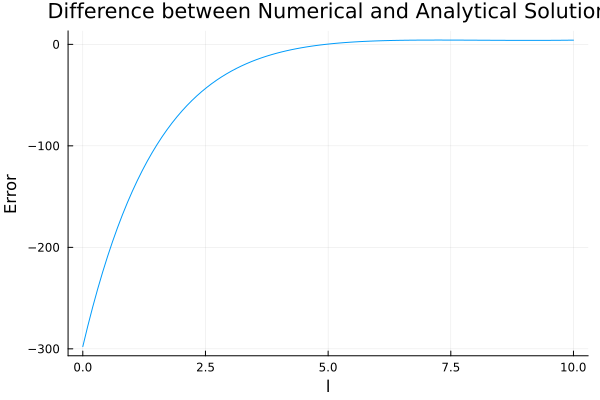
\includegraphics[width=7cm]{../figs/ex1_err_100.png}
\centering
\caption{Distance between the solutions at each mesh point for a mesh size of 0.1 cm.}
\end{figure}

Flux values from the numerical solver at the following locations (4 significant digits):\\
Flux value at $0^+ = 11979.0980 cm^{-2} s^{-1}$: \\
Flux value at $x_0 = 17.732 cm^{-2} s^{-1}$: \\


\begin{figure}[h]
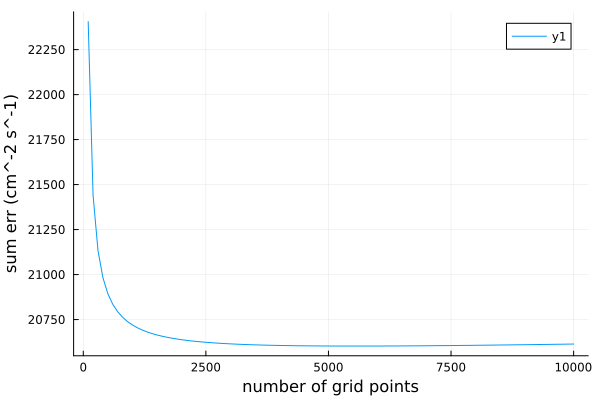
\includegraphics[width=7cm]{../figs/sum_errors.png}
\centering
\caption{Evolution with mesh size of the absolute error of $\Phi(x_0)$.}
\label{sumerr}
\end{figure}
\begin{figure}[h]
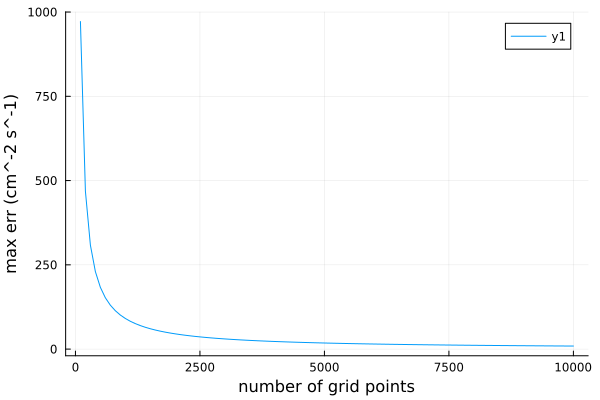
\includegraphics[width=7cm]{../figs/max_errors.png}
\centering
\caption{Evolution with mesh size of the absolute error of $\Phi(x_0)$.}
\label{maxerr}
\end{figure}

% Add two sentences describing what you see in \ref{sumerr} and a possible explanation 
In figure \ref{sumerr} you can see the sum of the errors and in \ref{maxerr} you can see the maximum deviation from the reference solution.


%%%%%%%






\end{document}
